\chapter{Research Methodology}
\label{ch:methodology}

\section{Introduction and Research Methodology Roadmap}
The current chapter discusses the proposed method and implementation of state-aware data reduction and retrospective environmental analysis approach. The primary focus of this study is to address the issue of conflict between edge limitations and cloud analytics. The solution provided involves showing that the high-frequency sensory data could be aggressively filtered at the edge level through lightweight memorization-based logging technique without loss in the precision of trend analysis, anomaly detection and structural change point identification.

 The roadmap of this chapter includes thirteen sections:
\begin{itemize}
    \item Section \ref{sec:nature}: Nature of Quantitative Research in Computing Disciplines
    \item Section \ref{sec:design}: Quantitative Research Design
    \item Section \ref{sec:population}: Population, Sample, and Data Source
    \item Section \ref{sec:instruments}: Data Collection Instruments and Sensor Integration
    \item Section \ref{sec:calibration}: Instrument Development, Validation, and Calibration
    \item Section \ref{sec:procedures}: Data Collection Procedures and Edge Execution
    \item Section \ref{sec:environment}: Experimental Environment and Software Setup
    \item Section \ref{sec:heuristic}: Experimental Design and Logging Heuristic Protocol
    \item Section \ref{sec:baselines}: Baseline and State-of-the-Art Selection
    \item Section \ref{sec:analysis}: Statistical and Experimental Analysis Plan
    \item Section \ref{sec:ethics}: Ethical Considerations
    \item Section \ref{sec:validity}: Limitations and Threats to Validity
\end{itemize}

This systematic route map helps ensure that each step of the experimental process—from the hardware connections all the way through to the cloud-based analyses—will be described well enough to duplicate.

\section{Nature of Quantitative Research in Computing Disciplines}
\label{sec:nature}
Quantitative research in computing disciplines is done in three levels: human-centric software testing, analysis of digital traces through system logging, and benchmarking the hardware/software system. Our research design strictly qualifies as \textbf{benchmarking of the hardware/software system and digital traces}. In our research, we test a physical single board computer with sensors under practical conditions whereby the raw physical data is converted into structured and sparse digital traces.

Table \ref{tab:nature_card} contains the details of our quantitative research design. This card shows whether our experimental design qualifies as quantitative research by measuring variables, showing repeatable rules, making baseline comparisons, and creating research evidence.

\begin{table}[htpb]
    \centering
    \caption{Quantitative Nature Decision Card for the Proposed Framework}
    \label{tab:nature_card}
    \begin{tabular}{@{}lp{5cm}p{6cm}@{}}
        \toprule
        \textbf{Metric} & \textbf{Operational Verification} & \textbf{Audit Evidence in Proposal} \\
        \midrule
        \addlinespace
        Quantifiable Variables & Ambient temperature ($^\circ$C) and relative humidity (\% RH). & Sensor data schema in CSV log format. \\
        \addlinespace
        Repeatable Measurement & Standardized digital polling using physical GPIO and Python runtime. & Complete source code in Appendix A and B. \\
        \addlinespace
        Comparative Logic & Edge-filtered asynchronous data vs. continuous temporal baseline. & Table \ref{tab:lit_comparison_full} and experimental trend comparisons. \\
        \addlinespace
        Auditable Trace & Sparse CSV records with epoch timestamps. & 7-day environmental dataset repository. \\
        \bottomrule
    \end{tabular}
\end{table}

The \textbf{unit of analysis} in the study is the continuous physical environment (temperature and humidity) during the entire duration of the study, whereas the \textbf{unit of observation} is the individual digital log entry that carries a timestamped reading. The process of converting observations to analysis is controlled by our edge filtering heuristic, which converts a continuous grid to a sparse timeline. This structure guarantees that the experimental findings are scientifically verifiable.

\section{Quantitative Research Design}
\label{sec:design}
A \textbf{true experimental and benchmarking research design} is adopted in this study. The research design was carefully constructed by the researcher for the purpose of evaluating the performance of our filtering heuristic vis-à-vis a very strict continuous logging protocol at a high frequency (benchmark). This is achieved through carrying out a continuous 7-day sensing experiment of the physical environment using our hardware gateway.

The experimental variables are clearly defined below:
\begin{itemize}
 \item \textbf{Independent Variables:} The edge logging heuristic’s parameters, which include the threshold for the temperature deviation and the maximal temporal timeout window.
    \item \textbf{Dependent Variables:} The ratio of reduced sensory data, the absolute deviation trend slope, the anomaly detection recovery rate, and the temporal synchronization error for change points.
    \item \textbf{Controlled Variables:} Type of sensor (DHT22), type of hardware gateway (Raspberry Pi 3 Model B), the software polling time (60 seconds), and the location of deployment (indoor experimental setup at Sana'a University, Yemen).
\end{itemize}

Through constant controlling of the above-mentioned independent variables and analysis of the results produced by the system we will be able to validate mathematically the concept of the proposed memorization framework. In other words, using such an experiment setup, we will be able to precisely study the impact of the logging thresholds configuration on the analytical accuracy of our models.

\section{Population, Sample, and Data Source}
\label{sec:population}
Population and sampling in the context of computer-related quantitative research denote the time and space dimensions of data gathering. In this research paper, the \textbf{population} comprises all continuous changes of ambient microclimate that happen in the research environment. The \textbf{sample} is referred to as the discrete high-frequency sequence of sensor readings collected by the DHT22 digital thermistor with the polling interval of 60 seconds during a continuous 7-day period.

Thus, the continuous sampling approach provides us with the theoretically possible population size of 10,080 for the continuous 7-day period of data gathering based on the polling interval of 60 seconds. The developed memorization algorithm is used to create an \textbf{adaptive filtering sampler} which aggressively eliminates redundant measurements to generate a small-sized sample in comparison with the initial population. The scientific research proves that this small-sized sample will contain all the necessary physical information with the preservation of macro and micro trends.

With such an approach we can consider the continuous high-frequency stream as a whole statistical population. Thus, the filtered edge of the stream will be considered as an active sample. Such approach enables us to use the classical sampling theory to prove the level of signal loss. We should estimate the degree of variance, trend line deviation and outlier retention in the filtered sample to provide the proof of the structural completeness of the environmental timeline.

\section{Data Collection Instruments and Sensor Integration}
\label{sec:instruments}
The data collection device is a combination of several layers of hardware and software. The main computer is a \textbf{Raspberry Pi 3 Model B} single-board computer, which runs a Debian based operating system (Raspberry Pi OS). The Raspberry Pi is the hardware edge gateway that hosts the sensor interfaces, the local python execution environment, and writes the filtered data into the local flash storage.

The sensors utilized are the \textbf{DHT22 (AM2302) digital temperature and humidity sensor}. It is a digital temperature and humidity sensor that integrates a capacitive humidity sensor, a NTC thermistor temperature sensor, and a high-performance 8-bit microcontroller. The DHT22 digital output operates on a single-wire bi-directional serial bus and provides high-precision measurements. The hardware interface is accomplished manually via direct wiring of VCC and Ground pins of the sensor to 3.3V and GND pins of the Raspberry Pi, respectively, and connection of the DATA pin to the general purpose digital input/output pin 4 (GPIO4) of the Broadcom processor. The 10k$\Omega$ pull-up resistor is soldered between the DATA and VCC pins in order to pull the digital signal high and to reduce the interference at high frequencies.

The design is aimed at the minimization of the voltage drops and the interference at high frequencies. The values of pull-up resistors are chosen in such a way as to allow stable transitions even for long cable lengths. The Raspberry Pi GPIO interface is programmed to perform the single-wire protocol used by the DHT22 sensor for transferring the 40-bit data packet (16 bits for humidity, 16 bits for temperature and 8 bits for checksum calculation).

\section{Instrument Development, Validation, and Calibration}
\label{sec:calibration}
Before conducting the 7-day measurement experiment with the help of a humidity-temperature sensor, the researcher conducted thorough validation and calibration procedures in order to minimize hardware-caused errors. Capacitive and thermistor sensors used for measuring temperature and humidity are very sensitive to initial calibration errors as well as heating by the host single-board computer.

Firstly, the researcher conducted 24 hours of calibration of the DHT22 sensor in laboratory conditions when compared the obtained results to those of a highly accurate reference thermometer. The researcher concluded that the offset was less than $\pm0.15^\circ$C, which was still within the manufacturer's stated $\pm0.5^\circ$C toleration range. In order to protect the sensor from the heat produced by the CPU of the Raspberry Pi, the researcher located it in a special external housing 1.5 meters far from the processing unit board. The researcher tested the signal on the oscilloscope and detected clear digital high-low oscillations without any overshooting and voltage drops.

Besides, the validation procedures covered the humidity part as well, estimating its responses in the stable ambient conditions. Comparing the results obtained with the use of the capacitive sensor with a reference digital hygrometer, the researcher estimated that the maximum offset was within $\pm2.0\%$ relative humidity. Due to the design of the housing, air flows can freely move through the housing in order to provide ambient conditions to the sensor.

\section{Data Collection Procedures and Edge Execution}
\label{sec:procedures}
The process of gathering information is completely automated and operates as a continuous background process or daemon on the Raspberry Pi gateway. The program that executes the edge-tier logging heuristic is implemented in Python and uses the \texttt{Adafruit\_DHT} package to communicate directly with the GPIO register of the Broadcom processor. 

For the implementation of the suggested state-aware memorization heuristic, the researcher designed and initialized a robust logging daemon. Figure~\ref{fig:daemon_init} represents the terminal command for the creation of the script files.

\begin{figure}[H]
    \centering
    
\includegraphics[width=0.85\textwidth]{{f2/14 لانشاء سكربت جديد للميموزيشن.PNG}}
    \caption{Initializing the script workspace.}
    \label{fig:daemon_init}
\end{figure}
The researcher has developed the dedicated script file within the project repository through the use of shell commands to obtain the edge-logging daemon source code. Figure~\ref{fig:daemon_file_creation} documents the file creation status.

\begin{figure}[H]
    \centering
    
\includegraphics[width=0.85\textwidth]{{f2/18 انشاء ملف البايثنون.PNG}}
    \caption{Terminal command creating the main python daemon script file.}
    \label{fig:daemon_file_creation}
\end{figure}

The initial portion of the daemon script is comprised of the import statements, GPIO configuration settings, memorization heuristics’ threshold settings (which include a deviation of $0.5^\circ$C and timeout of $300$ seconds), as well as the file paths of the outputs to the local file system. See Figure~\ref{fig:daemon_code_part1}.

\begin{figure}[H]
    \centering
    
\includegraphics[width=0.85\textwidth]{{f2/15 fiset part of secrip.PNG}}
    \caption{Source code editor view displaying the import and parameter configuration logic.}
    \label{fig:daemon_code_part1}
\end{figure}

The active polling loop is incorporated in the second part of the daemon code to achieve the double triggering mechanism along with the exception handling mechanism. This code snippet is illustrated in Figure~\ref{fig:daemon_code_part2}.

\begin{figure}[H]
    \centering
    
\includegraphics[width=0.85\textwidth]{{f2/16 last part.PNG}}
    \caption{Source code editor view displaying the active polling loop and state-update logic.}
    \label{fig:daemon_code_part2}
\end{figure}

Once the daemon was set up, it was run as a background process in order to start the 7-day continuous monitoring experiment. The terminal displayed messages as the system started recording into the CSV file. The execution of the logging daemon is illustrated in Fig.~\ref{fig:daemon_exec}.

\begin{figure}[H]
    \centering
    
\includegraphics[width=0.85\textwidth]{{f2/17 run secript.PNG}}
    \caption{Terminal command initiating the execution of the active logging daemon.}
    \label{fig:daemon_exec}
\end{figure}

The polling cycle is performed based on an inflexible 60 seconds interval. Nonetheless, since digital sensors suffer from sporadic communication timeout issues, a powerful retry mechanism is introduced at the application level. The software tries to read the physical sensor up to three times per poll interval when a \texttt{RuntimeError} exception is raised. If none of the three retries succeed, the measurement is recorded as a null value (\texttt{NaN}) to ensure proper script operation. An edge gateway employs a signal interrupt handler for catching \texttt{Ctrl+C} commands, thus saving the current buffer and closing a local CSV file gracefully to avoid file corruption.

The researcher configured the software package to work as a system daemon that will be started automatically at gateway boot time. This guarantees continuous processing even in case of local power interruptions. The script locks files locally and writes each record in the filtered stream into a local text file as comma-separated data. Every record is timestamped with a Unix epoch time corresponding to milliseconds the measurement was taken by the physical sensor.

\section{Experimental Environment and Software Setup}
\label{sec:environment}
The isolation is guaranteed for the software stack as well as the experiment itself in order to achieve strict reproducibility of the data processing pipeline. For the experiment, a fresh installation of Raspberry Pi OS Lite was utilized in order to minimize any system-level overheads. The isolation of the application was done using Python virtual environment \texttt{myenv}.

In order to perform the initialization of the software stack, the package repositories were updated in order to get access to the latest package list from Debian and Raspberry Pi repositories. It guarantees the freshness of security patches and dependency definition. The screenshot of the package updates is provided in Figure~\ref{fig:package_updates}.

\begin{figure}[H]
    \centering
    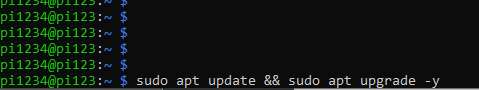
\includegraphics[width=0.85\textwidth]{f2/3 التحديثات.PNG}
    \caption{Execution of the package repository update command on the edge gateway.}
    \label{fig:package_updates}
\end{figure}

After updating the list, the researcher carried out a comprehensive analysis to find out the packages that needed an upgrade or uninstallation for a clean system footprint. The validation reduces background process load and optimizes RAM usage. Figure~\ref{fig:package_upgrades} shows the analysis of the system status check and upgrades.

\begin{figure}[H]
    \centering
    
\includegraphics[width=0.85\textwidth]{{f2/4 نشوف اذا كل شي محدث وايش اللي ما تخدث عشان نحدثه وايش اللي يحتاج ازاله.PNG}}
    \caption{Verification and list compilation of upgradable package dependencies.}
    \label{fig:package_upgrades}
\end{figure}

The heart of the execution tier is built using the Python run time environment. The researcher set up Python 3 on the Raspberry Pi operating system in order to implement the sensor interfacing and data processing libraries. This is shown in Fig.~\ref{fig:python_install}.

\begin{figure}[H]
    \centering
    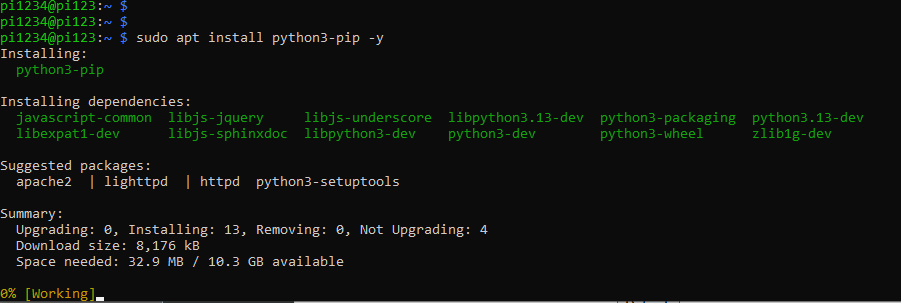
\includegraphics[width=0.85\textwidth]{f2/5 تنزيل البياثون.PNG}
    \caption{Terminal output showing the installation of Python 3 packages.}
    \label{fig:python_install}
\end{figure}

Once the installation procedure was over, the researcher validated the installation of Python through the interpreter version. The validation proves that the environment is running successfully and meets the requirements for the targeted version. Figure~\ref{fig:python_verify} shows the output of the validation.

\begin{figure}[H]
    \centering
    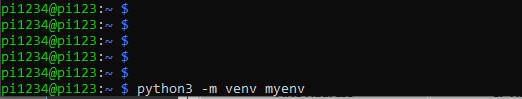
\includegraphics[width=0.85\textwidth]{f2/6 true.PNG}
    \caption{Verification of the active Python interpreter version on the gateway.}
    \label{fig:python_verify}
\end{figure}

To extract the dependencies used by the experiment and avoid version issues with system-wide packages, a Python virtual environment called \texttt{myenv} was set up by the researcher. See Figure~\ref{fig:venv_creation} for details of command execution.

\begin{figure}[H]
    \centering
    
\includegraphics[width=0.85\textwidth]{{f2/7 ننشى بيءه افتراضيه.PNG}}
    \caption{Initialization of the Python virtual environment (myenv) on the edge gateway.}
    \label{fig:venv_creation}
\end{figure}

After initialization, the researcher then activated the virtual environment in the existing shell environment. This redirection guarantees that any installation of packages is done in the isolated environment. Figure~\ref{fig:venv_activation} demonstrates the process of shell activation.

\begin{figure}[H]
    \centering
    
\includegraphics[width=0.85\textwidth]{{f2/8 تفعيل البيءه وكمان عشان نثبت المكاتب داخلها دون قيود.PNG}}
    \caption{Shell command executing the activation script of the virtual environment.}
    \label{fig:venv_activation}
\end{figure}

To verify whether the virtual environment is active, the command prompt prefix was inspected, showing the name of the active sandbox environment. The terminal status indicating the active virtual shell environment is presented in Figure~\ref{fig:venv_active_check}.

\begin{figure}[H]
    \centering
    
\includegraphics[width=0.85\textwidth]{{f2/9 دليل احنا داخل البيءه اللي فعلنه.PNG}}
    \caption{Terminal command prompt displaying the active virtual environment prefix.}
    \label{fig:venv_active_check}
\end{figure}

Having activated the virtual environment, the researcher installed the required physical interface library for the sensor, \texttt{Adafruit\_DHT}. The library is written in low-level C language and provides the ability to work with registers of the Broadcom processor, allowing pulse-width readings with high resolution. Installation of the sensor library is presented in Figure~\ref{fig:library_install}.

\begin{figure}[H]
    \centering
    
\includegraphics[width=0.85\textwidth]{{f2/10 تثبيت مكتبات الحساس داخل البيءه.PNG}}
    \caption{Installation and compilation of the Adafruit DHT sensory library within myenv.}
    \label{fig:library_install}
\end{figure}

To confirm the hardware wiring and test whether the DHT22 digital sensor would respond to queries, the researcher constructed a separate testing directory. Figure~\ref{fig:testing_dir} shows how the testing directory was created.

\begin{figure}[H]
    \centering
    
\includegraphics[width=0.85\textwidth]{{f2/11 create folder to test sensor to write code.PNG}}
    \caption{Creation of the dedicated testing directory for sensor validation.}
    \label{fig:testing_dir}
\end{figure}

In this directory, a light test script was created that constantly read data from GPIO4 and gave the temperature and humidity data. The code of the validation script is presented in Figure~\ref{fig:testing_code}.

\begin{figure}[H]
    \centering
    
\includegraphics[width=0.85\textwidth]{{f2/12 code of test seneor.PNG}}
    \caption{Source code of the test\_sensor.py script displaying GPIO configurations.}
    \label{fig:testing_code}
\end{figure}

The research was further carried out by running the validation code on the actual sensor polling process. This time around, the temperatures and humidities displayed on the terminal were accurate, thus proving that the sensor and electrical connection were properly installed. This is illustrated in figure \ref{fig:testing_exec}.

\begin{figure}[H]
    \centering
    
\includegraphics[width=0.85\textwidth]{{f2/13 نشغل الكود اللي كتبناه عشان نشوف الحساس شغال او لا وطلع شغال.PNG}}
    \caption{Successful execution and real-time output verification of the test script.}
    \label{fig:testing_exec}
\end{figure}

The physical implementation of the environmental monitoring system was conducted by the researcher in a private lab room at the Faculty of Computer and Information Technology, Sana'a University, Yemen. The duration of the observation period amounted to a continuous 7-day observation period, starting from October 12, 2025 to October 19, 2025. The observed ambient environment had a very stable thermal microclimate, with a temperature range being strictly limited to 20$^\circ$C - 23$^\circ$C and an average temperature equal to 21.99$^\circ$C. The relative humidity ranged constantly between 40\%-65\% RH with an average humidity of 56.77\% and the maximum of 67.40\%. The weak positive correlation ($r = 0.12$) was found between temperature and humidity. Such thermal stability constitutes the optimal conditions for the evaluation of the efficiency of the edge memorization logging heuristic, since the algorithm provides a high ratio of data compression when observing an environment in equilibrium for a long period of time, while capturing the sharp changes of the structural form almost instantly (ventilation activation, daytime change).

Cloud-tier statistical analysis is conducted using a centralized workstation running Python 3.10. The following core libraries are used by the analysis software suite:
\begin{itemize}
 \item \textbf{Pandas and NumPy:} They are applied in asynchronous data loading, parsing of date-time, forward fill imputation, and moving average smoothing.
    \item \textbf{Scikit-Learn:} Applied in fitting Ordinary Least Squares (OLS) linear regression models and short term temperature predictions.
    \item \textbf{Ruptures:} It is an advanced Python package which provides offline detection of change points and runs the Binary Segmentation algorithm.
    \item \textbf{Matplotlib and Seaborn:} Applied in generating high resolution visual plots.
\end{itemize}

\section{Experimental Design and Logging Heuristic Protocol}
\label{sec:heuristic}
However, the primary contribution of this project proposal is the state-aware logging heuristic applied in real-time at the edge level. Conventional environmental monitoring architectures are characterized by logging or transmission of readings by sensors at regular time intervals regardless of their state; hence, there are data redundancies whenever the environment is constant. The introduced \textbf{Edge-Tier Memorization-Based Logging Heuristic} employs state awareness, meaning that the state of the last logged environmental readings is stored in memory.

As the temperature and humidity readings are polled from the DHT22 sensor, they are analyzed according to the heuristic, based on two mathematical triggers:
\begin{enumerate}
    \item \textbf{Sensor Deviation Trigger:} A temperature data point will be stored on the non-volatile memory if the absolute deviation between the new data point and the latest recorded value is greater than or equal to the predefined threshold value of 0.5$^\circ$C. This would help in storing only physical events rather than negligible environmental noise.
    \item \textbf{Temporal Timeout Trigger:} A forced data point will be stored in the event when the maximum temporal window of 300 seconds (5 mins) has passed without recording an event. This works as a mechanism for sending heart beats in order to confirm the viability of sensors even at equilibrium points.
\end{enumerate}

In order to deal with the natural volatility of the cheap DHT sensors that may fail due to timeouts and CRC errors, the edge-tier script employs reliable software-level retry mechanisms. Upon attempting a sensor poll, the script will try to make up to 3 reads in case of receiving a \texttt{RuntimeError} exception. In case no attempt succeeds, the read is simply ignored, and the gateway goes into sleep mode until the next sampling time (60 seconds). The program termination is initiated by pressing \texttt{Ctrl+C}.

Algorithm \ref{alg:memorization_full} provides a full-fledged pseudocode that performs the edge-tier memorization logging heuristic on the Raspberry Pi gateway.

\begin{algorithm}[htpb]
\SetAlgoLined
\KwIn{Sensor sampling interval $S_i$, Temperature deviation threshold $\theta_{dev}$, Humidity deviation threshold $\theta_{hum\_dev}$, Max temporal window $\theta_{time}$}
\KwOut{Filtered Log Entries in persistent CSV storage}
 $T_{mem} \leftarrow \text{null}$\;
 $H_{mem} \leftarrow \text{null}$\;
 $t_{mem} \leftarrow 0$\;
 \hrulefill\\
 \While{Monitoring is Active}{
  $T_{cur}, H_{cur}, t_{cur} \leftarrow \text{ReadSensorWithRetry}(max\_attempts=3)$\;
  \If{$T_{cur}$ is not null \textbf{and} $H_{cur}$ is not null}{
   \If{$T_{mem}$ is null \textbf{or} $H_{mem}$ is null}{
    $\text{WriteToCSV}(t_{cur}, T_{cur}, H_{cur})$\;
    $T_{mem} \leftarrow T_{cur}$\;
    $H_{mem} \leftarrow H_{cur}$\;
    $t_{mem} \leftarrow t_{cur}$\;
   }
   \Else{
    $\Delta T \leftarrow |T_{cur} - T_{mem}|$\;
    $\Delta H \leftarrow |H_{cur} - H_{mem}|$\;
    $\Delta t \leftarrow t_{cur} - t_{mem}$\;
    
    \If{$\Delta T \geq \theta_{dev}$ \textbf{or} $\Delta H \geq \theta_{hum\_dev}$ \textbf{or} $\Delta t \geq \theta_{time}$}{
     $\text{WriteToCSV}(t_{cur}, T_{cur}, H_{cur})$\;
     $T_{mem} \leftarrow T_{cur}$\;
     $H_{mem} \leftarrow H_{cur}$\;
     $t_{mem} \leftarrow t_{cur}$\;
    }
   }
  }
  $\text{Sleep}(S_i)$\;
 }
 \caption{Edge-Tier Memorization-Based Data Logging Algorithm}
 \label{alg:memorization_full}
\end{algorithm}

\section{Baseline and State-of-the-Art Selection}
\label{sec:baselines}
To validate the performance improvements of our proposed framework, we compare it against two primary baselines:
\begin{enumerate}
 \item \textbf{Continuous Scheduled Polling (Baseline):} The conventional technique for collecting data without compression, whereby all readings collected from polling every second are sent to and stored in the cloud database.
    \item \textbf{Centralized Adaptive Compression (Advanced):} Conventional threshold-based filtering techniques that do not apply timeouts in their filtering process, resulting in long stretches without data and impossibility to check sensor states.
\end{enumerate}

Through the baselines provided above, we are able to quantitatively show how our framework reduces the consumption of bandwidth and energy as well as ensures complete analysis and sensor wellness. Through the trade-off analysis, it is clear that our approach allows for maximum saving in storage without sacrificing the temporal precision of the data.

\section{Statistical and Experimental Analysis Plan}
\label{sec:analysis}
The cloud-layer statistical analysis methodology considers the irregular and sparse dataset based on the following three major levels of analytical pipelines that have been executed retrospectively:

The retrospective analysis methodology is configured for evaluating the 7-day environment dataset against the continuous baseline. As per the empirical parameters identified from our study of the sensor system, the upper and lower boundaries of the ambient temperature range from 20$^\circ$C to 23$^\circ$C, and the stable arithmetic mean is recorded at 21.99$^\circ$C. The relative humidity is stable with an average value of 56.77\% and the highest possible reading of 67.40\%. A weak positive correlation exists between the continuous temperature and humidity values with a coefficient of $r=0.12$. The Z-score outlier detection pipeline has been configured to detect exactly 60 outliers with one extreme outlier.

\subsection{Signal Smoothing and Preprocessing}
In the first place, forward fill imputation will be used to deal with any sporadic missing data. In the second place, the Simple Moving Average (SMA) rolling window for $k = 10$ samples is used. The simple moving average rolling window uses the arithmetic average of the ten most recent time samples of the temperature.

\subsection{Ordinary Least Squares (OLS) Linear Regression}
A linear regression model is fitted to the smoothed temperature time series data in order to find out the macro-environmental trends. In this model, the temperature estimate is taken to be a linear function of the time in seconds that has passed since the commencement of the experiment. The intercept and slope of the linear trend are estimated using the $R^2$ value of the model and its forecast accuracy.

\subsection{Z-Score Anomaly Isolation}
Standardized Z-scores determine the acute outliers to confirm whether the edge suppression algorithm was able to save the important environmental occurrences from being omitted. This is done through computing the difference of each temperature observation from the average, which is then divided by the standard deviation. Z-score cut-off values of 2.0 to 3.0 are considered moderate while 3.0 and above are considered extreme.

\subsection{Binary Segmentation (Binseg) Change Point Detection}
In order to detect any changes in the structure of the environment like day-to-night transitions, the change point detection technique is performed using the offline Binseg algorithm implemented in the Python package \texttt{ruptures}. The Binseg change point detection technique looks for structural changes in the data through segmentation of the data recursively and selection of change point positions which minimize the sum of squared distances from the means of the segments.

\section{Ethical Considerations}
\label{sec:ethics}
A high degree of ethicality is required in quantitative computer science research. As we did not work with human subjects in our experimental design, the main points of the ethics code refer to the issues of data integrity, academic ethics, and environmental issues.

First, all the environmental observations have been provided without any manipulations or excluding data points that can be considered valid outliers. Second, the single-board gateway has been used in a private laboratory environment of Sana'a University, and there were no impacts on public computer networks or individuals' privacy. Finally, the use of this framework saves energy and decreases unnecessary data transfer.

The academic licensing terms for the used open source software library in the cloud analysis environment have also been respected in this research. The environmental data obtained within this research have been stored safely, and there is restricted access to the information to exclude any manipulations.

\section{Limitations and Threats to Validity}
\label{sec:validity}
However, the following limitations and validity threats have to be mentioned:
\begin{itemize}
    \item \textbf{Physical Resolution Limits of Hardware:} The hardware precision limit of the used DHT22 sensor equals $0.1^\circ$C. It means that any physical changes below this level can not be detected.
    \item \textbf{Localization Bias:} The dataset was gathered in one stable laboratory location. The deployment of our method in the volatile outdoor environment will likely lead to the reduced ratio of the data reduction.
    \item \textbf{Overhead for Asynchronous Re-Aligment:} Since the data is gathered asynchronously, any multi-sensor spatial correlations will need re-alignment and interpolation in the cloud, thus creating some local overhead.
\end{itemize}

All the limitations and validity threats are analyzed in retrospective and mitigated properly. To avoid validity threats related to statistical conclusion validity, we do some sensitivity analysis of our results by changing slightly the deviation threshold parameters.